%%%%%%%%%%%%%%%%%%%%%%%%%%%%%%%%%%%%%%%%%%%%%%%%%%%%%%%%%%%%%%%%%%%%%%%%
%    INSTITUTE OF PHYSICS PUBLISHING                                   %
%                                                                      %
%   `Preparing an article for publication in an Institute of Physics   %
%    Publishing journal using LaTeX'                                   %
%                                                                      %
%    LaTeX source code `ioplau2e.tex' used to generate `author         %
%    guidelines', the documentation explaining and demonstrating use   %
%    of the Institute of Physics Publishing LaTeX preprint files       %
%    `iopart.cls, iopart12.clo and iopart10.clo'.                      %
%                                                                      %
%    `ioplau2e.tex' itself uses LaTeX with `iopart.cls'                %
%                                                                      %
%%%%%%%%%%%%%%%%%%%%%%%%%%%%%%%%%%
%
%
% First we have a character check
%
% ! exclamation mark    " double quote  
% # hash                ` opening quote (grave)
% & ampersand           ' closing quote (acute)
% $ dollar              % percent       
% ( open parenthesis    ) close paren.  
% - hyphen              = equals sign
% | vertical bar        ~ tilde         
% @ at sign             _ underscore
% { open curly brace    } close curly   
% [ open square         ] close square bracket
% + plus sign           ; semi-colon    
% * asterisk            : colon
% < open angle bracket  > close angle   
% , comma               . full stop
% ? question mark       / forward slash 
% \ backslash           ^ circumflex
%
% ABCDEFGHIJKLMNOPQRSTUVWXYZ 
% abcdefghijklmnopqrstuvwxyz 
% 1234567890
%
%%%%%%%%%%%%%%%%%%%%%%%%%%%%%%%%%%%%%%%%%%%%%%%%%%%%%%%%%%%%%%%%%%%
%
\documentclass[12pt]{iopart}
\newcommand{\gguide}{{\it Preparing graphics for IOP journals}}
%Uncomment next line if AMS fonts required
\usepackage{iopams} 
\usepackage{graphicx, subfigure}

\begin{document}

\title[]{Shear Flow of Cubic Blue Phases in Confined Geometries}

\author{O. Henrich$^{1,3}$, K. Stratford$^2$, D. Marenduzzo$^3$, P.V. Coveney$^1$ and M.E. Cates $^3$}

\address{$^1$ Centre for Computational Science, University College London, UK\\$^2$ Edinburgh Parallel Computing Centre, University of Edinburgh, UK\\$^3$ School of Physics and Astronomy, University of Edinburgh, UK}
\ead{o.henrich@ucl.ac.uk}

\begin{abstract}
\end{abstract}

%Uncomment for PACS numbers title message
%\pacs{00.00, 20.00, 42.10}
% Keywords required only for MST, PB, PMB, PM, JOA, JOB? 
%\vspace{2pc}
%\noindent{\it Keywords}: Article preparation, IOP journals
% Uncomment for Submitted to journal title message
%\submitto{\JPA}
% Comment out if separate title page not required
\maketitle

\section{Introduction}
% Put \label in argument of \section for cross-referencing
%\section{\label{}}
\section{Model and Methods}

%Our approach is based on a well-established model for hydrodynamics of cholesteric liquid crystals \cite{Beris:1994,Olmsted:1999} that describes the order structure of the liquid crystal by a traceless, symmetric tensor order parameter ${\bf Q}({\bf r})$. 
%In uniaxial approximation the tensor order paramter is given by $Q_{\alpha \beta}=\langle n_\alpha n_\beta - 1/3\; \delta_{\alpha\beta}\rangle$, whereas ${\bf n}$ represents the local orientation of the liquid crystal molecules and brackets indicate mesoscopic averaging over a large number individual molecules.
%Its largest eigenvalue $\frac{2}{3}q$ with $0<q<1$ characterizes the degree of order around the corresponding axis. 
%The equilibrium properties of the system are determined by a Landau-de Gennes free energy density $f$ and the functional ${\cal F}[Q]=\int d^3{\bf r} f({\bf Q})$.
%The free energy density consists of two different parts, namely a bulk contribution $f_b$ and a gradient term $f_g$.

%\begin{eqnarray}
%f_b&=&\frac{A_0}{2}\left(1-\frac{\gamma}{3}\right) Q_{\alpha \beta}^2-\frac{A_0 \gamma}{3}Q_{\alpha \beta} Q_{\beta \gamma} Q_{\gamma \alpha}+\frac{A_0 \gamma}{4}(Q_{\alpha \beta}^2)^2\nonumber\\
%f_g&=&\frac{K}{2}(\varepsilon_{\alpha\gamma\delta} \partial_\gamma Q_{\delta\beta}+2 q_0 Q_{\alpha \beta})^2+\frac{K}{2}(\partial_\beta Q_{\alpha \beta})^2\label{eqn1}
%\end{eqnarray}

%The first term contains the bulk-free energy constant $A_0$ and the inverse temperature $\gamma$ and features a the first-order transition from the isotropic to the ordered phase at $\gamma>2.7$.
%The second part comprises the elastic contributions to the free energy due to splay-, bend- and twist-deformations and assume for simplicity that they have all the same elastic constant $K$.
%The pitch length $p$ of the cholesteric liquid crystal is related to the wavervector $q_0=2\pi/p$.
%In order to specify a thermodynamic state it is useful to introduce two dimensionless quantities, the effective temperature $\tau$ and chirality $\kappa$.
%They are given by 

%\begin{eqnarray}
%\tau&=&\frac{27(1-\gamma/3)}{\gamma}\nonumber\\
%\kappa&=&\sqrt{\frac{108 K q_0^2}{A_0 \gamma}}\nonumber,
%\end{eqnarray}

%whereas the chirality qqnatifies the ratio between gradient and bulk free energy.\\
%The equation of motion of the tensor order parameter reads

%\begin{equation}\label{}
%\left(\partial_t+ u_\alpha \partial_\alpha \right){\bf Q} - {\bf S}({\bf W},{\bf Q}) = \Gamma {\bf H}.
%\label{eqn2}
%\end{equation}

%The first term on the lefthand side of Eq.(\ref{eqn2}) is a material derivative, which describes the rate of change of a quantity moving along with the flow.
%The second term accounts for the rate of change due to velocity gradients $W_{\alpha \beta}=\partial_\beta u_\alpha$:

%\begin{eqnarray}
%{\bf S}({\bf W}, {\bf Q}) &=& (\xi {\bf A} + {\boldsymbol \Omega})({\bf Q}+\frac{\bf I}{3})\nonumber\\
%& &\hspace*{-1.5cm}+ ({\bf Q}+\frac{\bf I}{3})(\xi {\bf A}  - {\boldsymbol \Omega})-2 \xi ({\bf Q}+\frac{\bf I}{3})Tr({\bf Q W}),
%\label{eqn3}
%\end{eqnarray}

%where $Tr$ denotes the trace operation and ${\bf A}=({\bf W}+{\bf W}^T)/2$ and ${\boldsymbol \Omega}=({\bf W}-{\bf W}^T)/2$ are the symmetric and antisymmetric part of the velocity gradients, respectively.
%The molecular details of the liquid crystal such as the aspect ratio of its mesogens are embodied in the constant $\xi$, also know as the tumbling parameter.
%The righthand side relates the rate of change to the molecular field, which is a functional derivative of $\cal F$ that preserves the tracelessness of $\bf Q$.

%\begin{equation}
%{\bf H}=-\frac{\delta {\cal F}}{\delta {\bf Q}}+\frac{\bf I}{3}\, Tr\left(\frac{\delta {\cal F}}{\delta {\bf Q}}\right).
%\label{eqn4}
%\end{equation}

%The rotational diffusion constant $\Gamma$ is proportional to the inverse of the rotational viscosity $\gamma_1=2 q^2/\Gamma$.\\
%The time evolution of density and velocity are goverend by the continuity equation Eq. (\ref{eqn5}) 

%\begin{eqnarray}
%\partial_t \rho + \partial_\alpha (\rho u_\alpha)=0
%\label{eqn5}
%\end{eqnarray}

%and the Navier-Stokes equation Eq. (\ref{eqn6})

%\begin{eqnarray}
%\partial_t u_\alpha +\rho \,u_\beta \partial_\beta u_\alpha&=&\partial_\beta \Pi_{\alpha \beta}\nonumber\\
%&+&\hspace*{-2cm}\eta\, \partial_\beta \{ \partial_\alpha u_\beta + \partial_\beta u_\alpha +(1+3\frac{P_0}{\partial \rho} )\partial_\mu u_\mu \delta_{\alpha \beta})\}. 
%\label{eqn6}
%\end{eqnarray}

%At low flow rates the fluid can be considered as incompressible, so that the last term on the righthand side of Eq. (\ref{eqn6}) can be safely neglected.
%The pressure tensor reads explicitely

%\begin{eqnarray}
%\Pi_{\alpha \beta}&=&P_0-\xi H_{\alpha \gamma}\left(Q_{\gamma \beta} +\frac{1}{3} \delta_{\gamma \beta}\right)-\xi \left(Q_{\alpha \gamma} +\frac{1}{3} \delta_{\alpha \gamma}\right) H_{\gamma \beta}\nonumber\\
%&+& 2 \xi  \left(Q_{\alpha \beta} +\frac{1}{3} \delta_{\alpha \beta}\right) Q_{\gamma \nu} H_{\gamma \nu}-\partial_\alpha Q_{\gamma \nu} \frac{\delta{\cal F}}{\delta \partial_{\beta} Q_{\gamma \nu}}\nonumber\\
%&+&Q_{\alpha \gamma}H_{\gamma \beta}-H_{\alpha \gamma} Q_{\gamma \beta}.
%\label{eqn7}
%\end{eqnarray}

%It comprises the terms that give rise to an additional stress in the ordered state.
%In the isotropic state when ${\bf Q}\equiv 0$ Eq. (\ref{eqn7}) is reduced to the scalar pressure, which is constant to a very good approximation.\\ 
%The system of coupled partial differential equations is solved by means of a hybrid scheme \cite{Denniston:2004, Marenduzzo:2008} that uses a lattice Boltzmann algorithm with predictor-corrector scheme for the hydrodynamic equations (\ref{eqn5}) and (\ref{eqn6}) and a finite difference scheme for the tensor order parameter equation (\ref{eqn2}).


\section{Results and Discussion}

\begin{figure}[h]
\centering
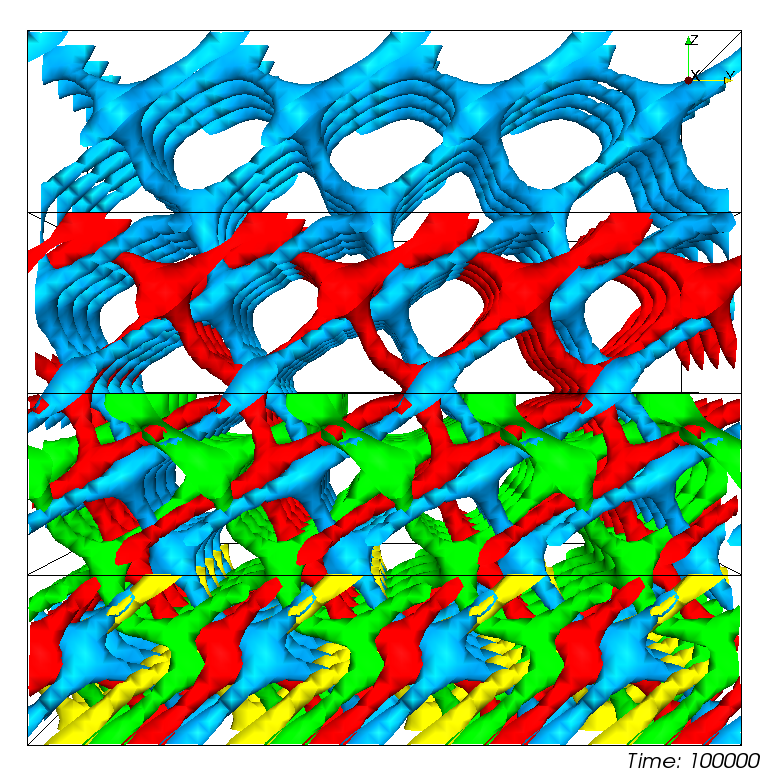
\includegraphics[width=0.45\textwidth]{disc_bp2_t-0o5_k2o0_100k_x.png}
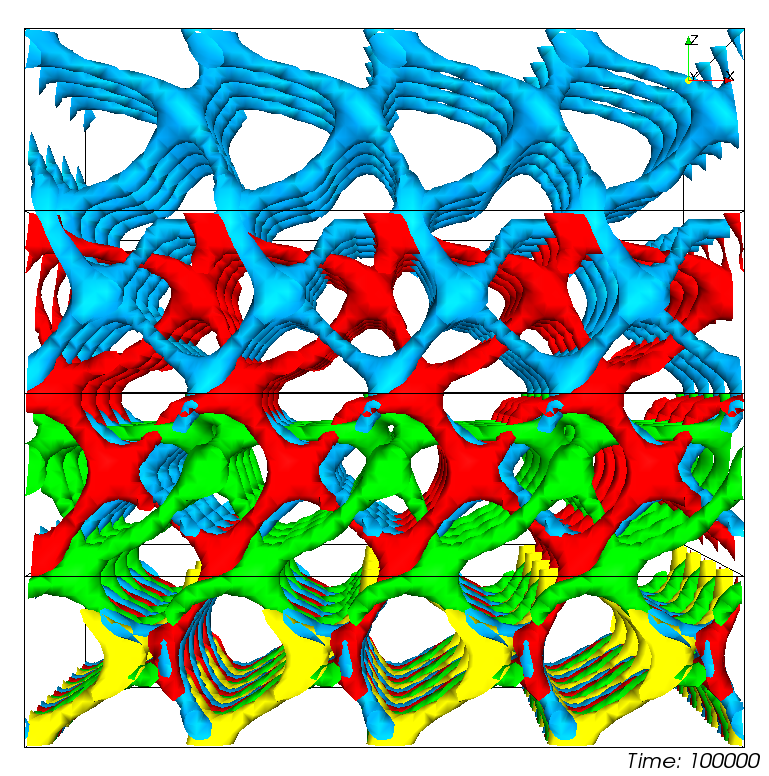
\includegraphics[width=0.45\textwidth]{disc_bp2_t-0o5_k2o0_100k_y.png}\\
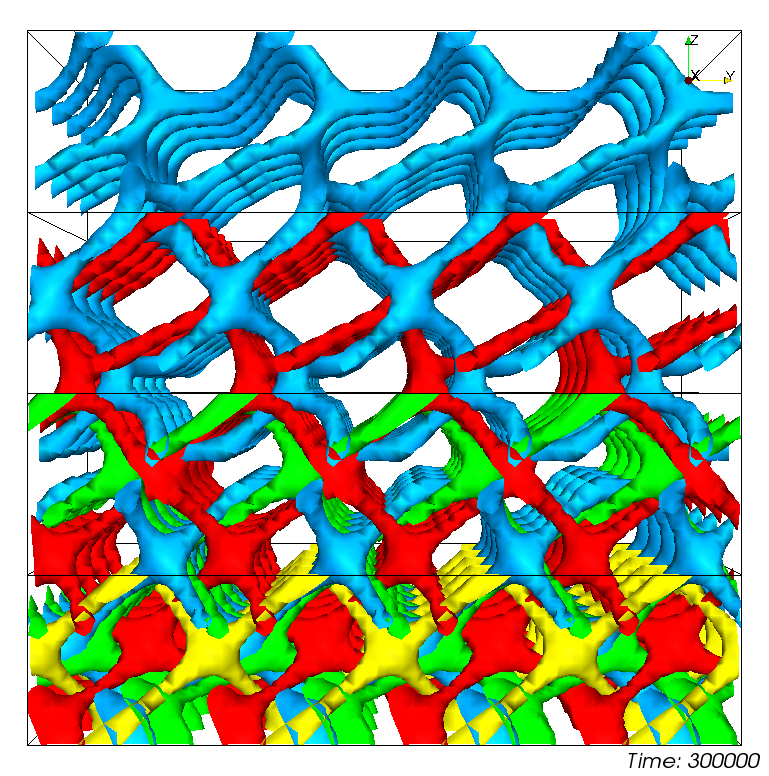
\includegraphics[width=0.45\textwidth]{disc_bp2_t-0o5_k2o0_300k_x.png}
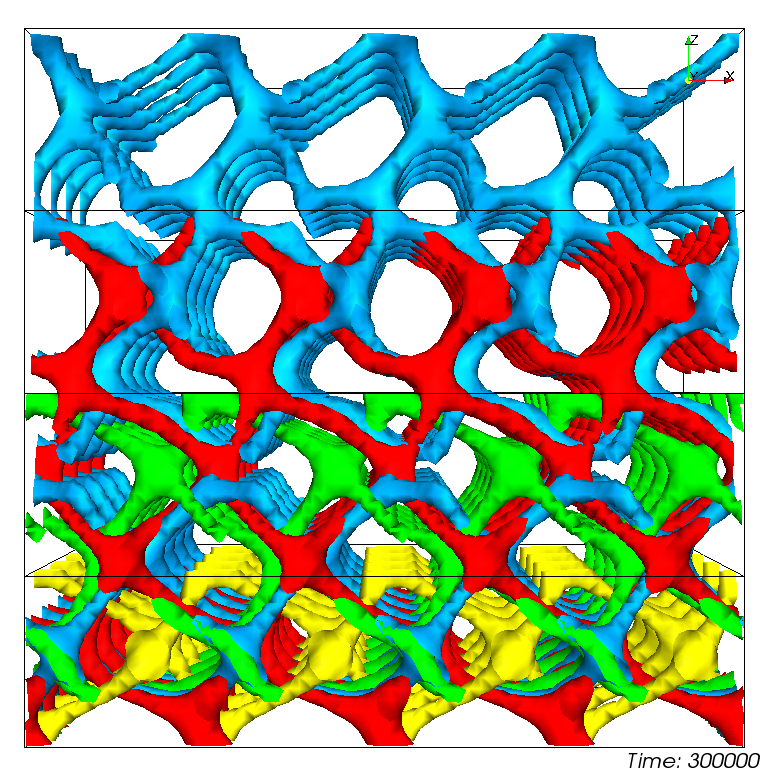
\includegraphics[width=0.45\textwidth]{disc_bp2_t-0o5_k2o0_300k_y.png}
\caption{}
\label{fig1}
\end{figure}

\begin{figure*}[h]
\centering
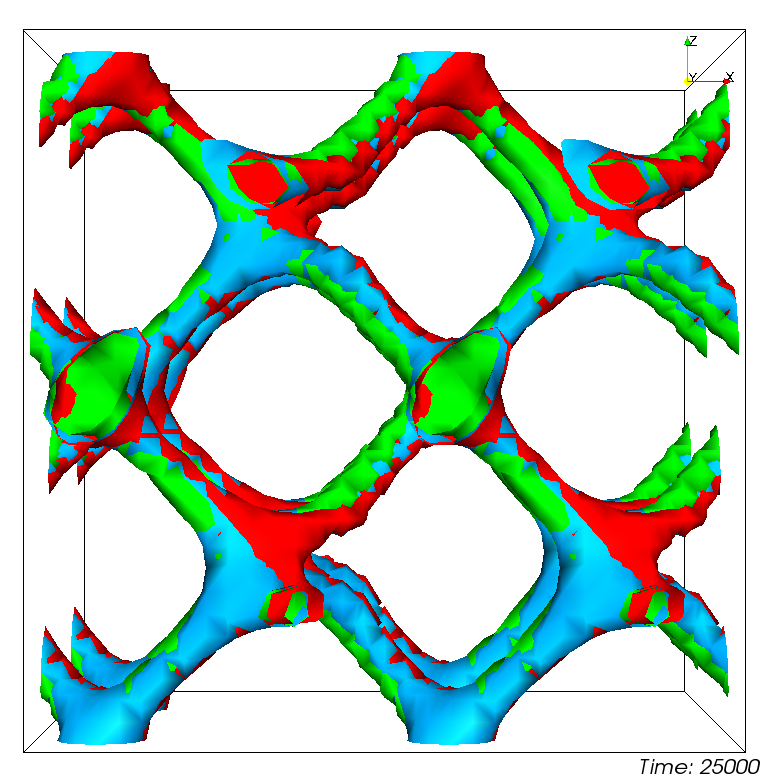
\includegraphics[width=0.3\textwidth]{disc_bp2_tk_scan_25k.png}
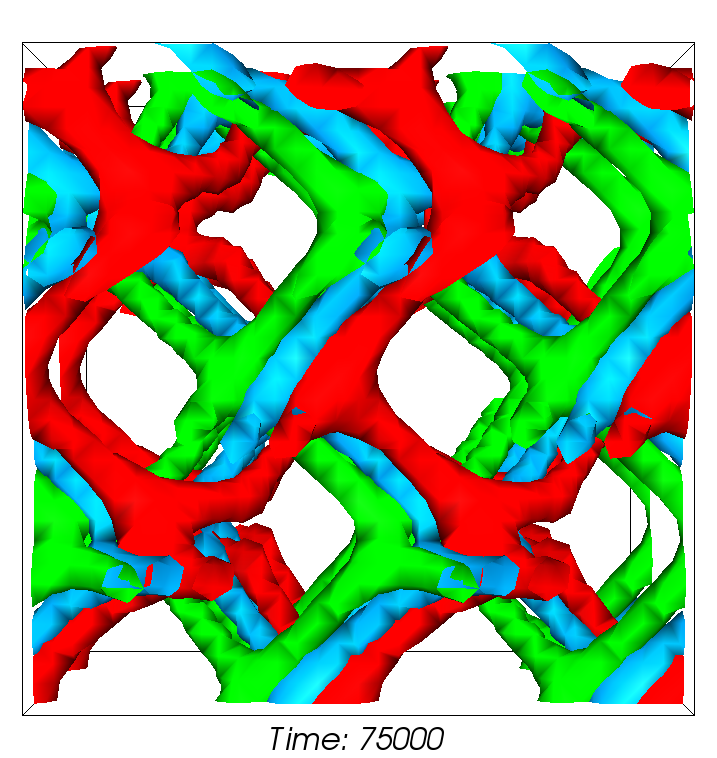
\includegraphics[width=0.3\textwidth]{disc_bp2_tk_scan_75k.png}
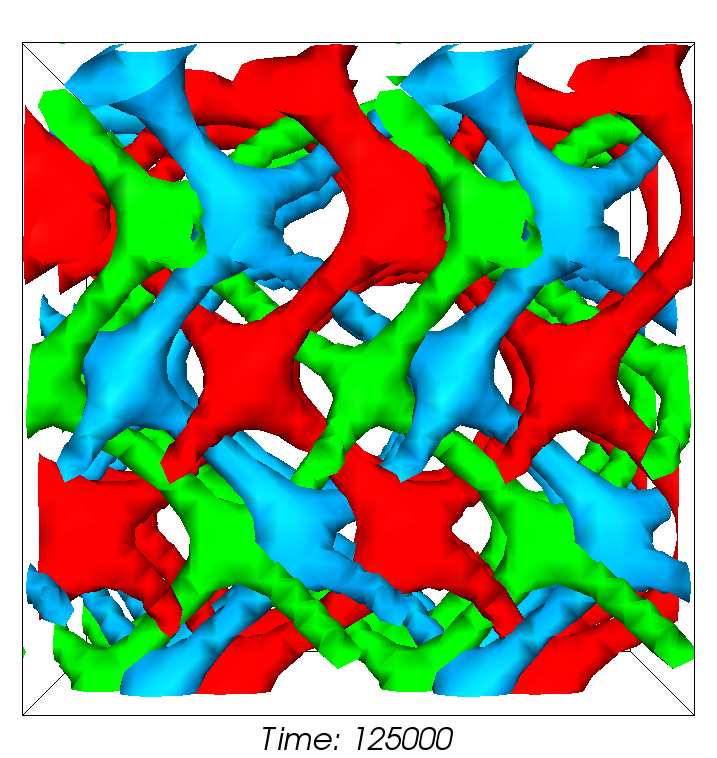
\includegraphics[width=0.3\textwidth]{disc_bp2_tk_scan_125k.png}
\caption{}
\label{fig2}
\end{figure*}

\begin{figure*}[h]
\centering
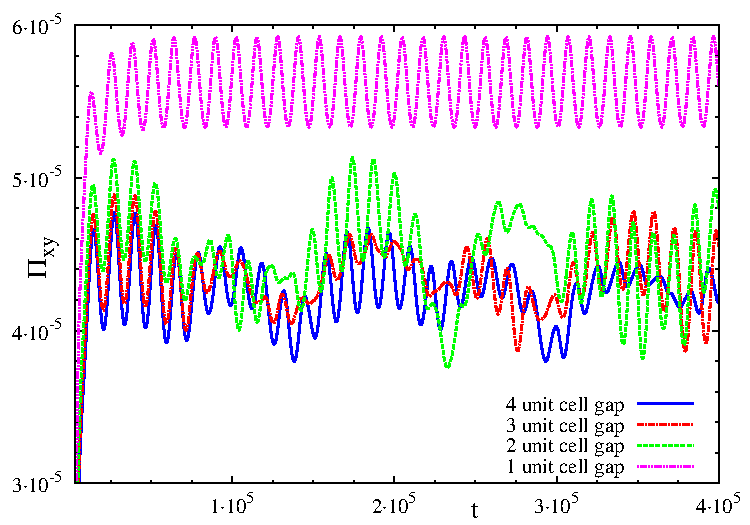
\includegraphics[width=\textwidth]{stress_bp2_fbc.pdf}
\caption{}
\label{fig3}
\end{figure*}

\begin{figure*}[h]
\centering
\begin{minipage}[b]{0.3\textwidth}
\subfigure[]{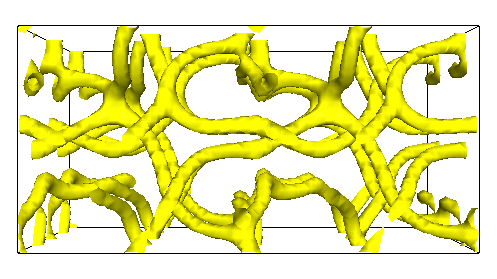
\includegraphics[width=\textwidth]{disc_bp1_t-0o5_k1o0_400k_1uc.png}}
\subfigure[]{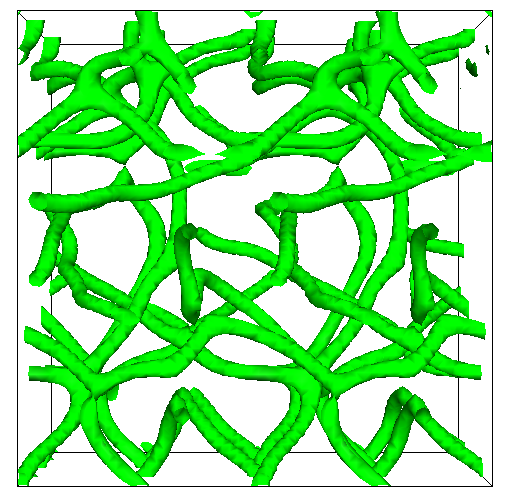
\includegraphics[width=\textwidth]{disc_bp1_t-0o5_k1o0_400k_2uc.png}}
\end{minipage}
\subfigure[]{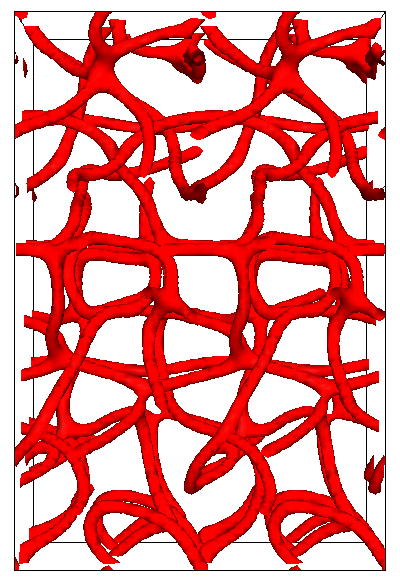
\includegraphics[width=0.3\textwidth]{disc_bp1_t-0o5_k1o0_400k_3uc.png}} 
\subfigure[]{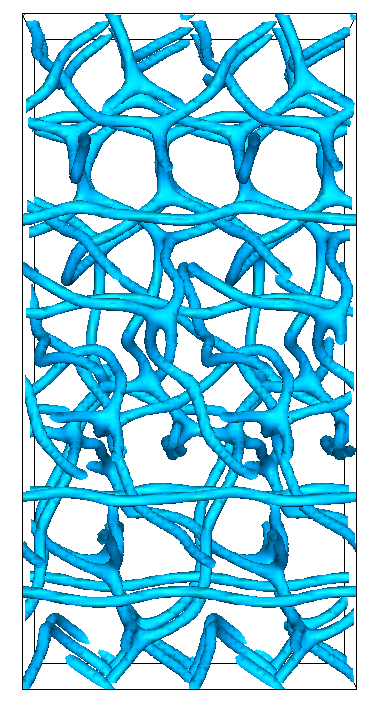
\includegraphics[width=0.3\textwidth]{disc_bp1_t-0o5_k1o0_400k_4uc.png}}
\caption{}
\label{fig4}
\end{figure*}

\begin{figure*}[h]
\centering
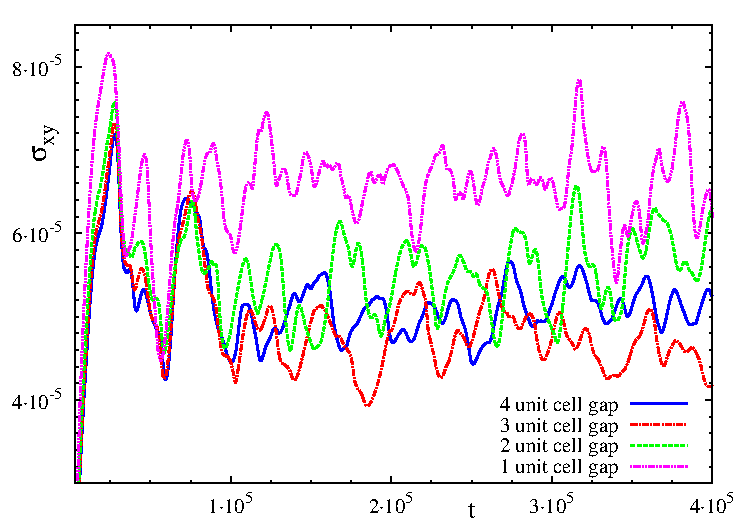
\includegraphics[width=\textwidth]{stress_bp1_fbc.pdf}
\caption{}
\label{fig5}
\end{figure*}

\section{Conclusions}

% If you have acknowledgments, this puts in the proper section head.
\ack
Thanks folks!

% Create the reference section using BibTeX:

\section*{References}
\bibliography{lmcproc}

\end{document}

